\documentclass{article}
\usepackage{tccml_iclr2025_conference}
\usepackage{graphicx}
\usepackage{url}
\usepackage{hyperref} % Load hyperref after natbib
\usepackage{amsmath}
\usepackage{colortbl} % For coloring table cells


% prev title: Exploring Multi-Model Ensembling Methods to Improve on Deep Learning Based Smoke Detection
\title{Improving Deep Learning-Based Wildfire\\ Smoke Plume Detection with a Multi-Model\\ Ensemble Approach}
\author{Author Name \\
Institution \\
\texttt{email@example.com}
}
\iclrfinalcopy
\begin{document}
\maketitle
% 3 PAGE MAXIMUM, WITH FIGURES, WITHOUT REFERENCES

% PREVIOUS ABSTRACT:
% \begin{abstract}
% With increasing occurrences of wildfires in recent years, effective and fast-delivering wildfire and smoke detection tools are needed to support hazard management and reduce risks to human health and environmental resources. The NOAA Geostationary Operational Environmental Satellites (GOES) provide high spatial and temporal resolution imagery of North America that can be used to detect the presence and density of smoke plumes. Recent advancements in computer vision have shown the capabilities of deep learning models to automate the semantic segmentation of high resolution images by training encoder-decoder networks on large labeled datasets. Additionally, ensemble methods can improve model generalization and prediction accuracy by combining the results of multiple models. We present an ensemble of deep learning models that produces representative predictions of where wildfire smoke plumes exist and their relative density (i.e. light, medium, heavy) in GOES imagery. Our results demonstrate that ensemble techniques can improve performance compared to using a single model. This multi-model data-driven ensemble is expected to support fire and hazard management by being able to automate the monitoring of smoke in real-time from satellite imagery.
% \end{abstract}

\begin{abstract}
With the increasing frequency and severity of wildfires, there is an urgent need for effective and rapid wildfire and smoke detection tools. Recent advancements in computer vision have demonstrated the potential of deep learning models, particularly neural networks, to automate the partitioning of high-resolution images into labelled segments. However, single-model approaches can struggle with generalization and accuracy in diverse conditions. To address these challenges, we propose creating an ensemble of deep learning models to produce accurate and representative predictions of wildfire smoke plumes and their relative density (light, medium, heavy) in Geostationary Operational Environmental Satellite (GOES) imagery. Our results indicate that this ensemble technique can significantly improve performance compared to using a single model. This multi-model ensemble is expected to support fire and hazard management by being able to automate the monitoring of smoke in real-time from satellite imagery, providing a valuable tool for air quality and fire hazard management in the face of worsening wildfires.
\end{abstract}

\section{Introduction}
% should i include this, to pertain to the climate change workshop? do i have room??? *** both these studies sitck to Western US
% Anthropogenic climate change drives warmer, drier conditions, leading to increased risk of severe wildfires \citep{cc-fire} \citep{climate-fire-risk}.
% from CCAI site: Each submission should make clear why the application has (or could have) a pathway to positive impacts regarding climate change.
% from CCAI site: Authors should clearly illustrate a pathway to climate impact, i.e., identify the way in which this work fits into broader efforts to address climate change. 
Wildfires increase smoke and particulate matter in the atmosphere, posing more risks of respiratory issues and other air quality-induced health problems in recent years \citep{wildfire-risk}. Effective and timely wildfire and smoke detection tools are thus essential for supporting hazard management and mitigating risks to human health. 

The National Oceanic and Atmospheric Administration (NOAA) Geostationary Operational Environmental Satellites (GOES) provide high spatial and temporal resolution imagery of North America \citep{GOESbook}, which can be leveraged to detect the presence and density of smoke plumes. The Hazard Mapping System (HMS) Fire and Smoke Product currently relies on human analysts to annotate the presence of smoke over North America using imagery from the GOES imagery \citep{hms}. However, this product is limited by the availability of human analysts, outputting annotations once to several times a day, and usually has a delay between smoke occurance and the annotation. To address this limitation in the availability of smoke data, we are leveraging advancements in deep learning to automate the detection of smoke from GOES imagery. Deep learning models, particularly encoder-decoder neural networks, have shown promise in automating the semantic segmentation (labelling images on a pixel-wise basis with multiple classes) of high-resolution images \citep{cv-segmentation-review}. By automating this task, we can enable more frequent and consistent detection of smoke plumes.

This proposal focuses on enhancing the capability of smoke detection with deep learning through the use of multi-model ensemble techniques. It has been shown for classification that ensemble methods that combine the predictions of multiple classifers can often perform better than a single classifer \citep{ensemble-ml}. Particularly, utilizing a diverse set of classifiers in an ensemble is important to achieve the improvement in performance \citep{ensemble-diversity}. In the neural network setting, combining the predictions of multiple independently-trained models can improve generalization and prediction accuracy of neural networks \citep{nn-ensemble}, \citep{nn-ensemble2}, \citep{nn-error-ens}. This approach aims to provide a more reliable and accurate tool for real-time monitoring of smoke, ultimately supporting fire and hazard management efforts and contributing to climate resilience and adaptation strategies.
% \citep{nn-error-ens} demonstrated the importance of the neural networks having independent errors, or "error diversity" for the ensemble to succeed. it also provided a mathematical basis (clustering of errors) for designing ensembles that contain error diversity between the models.

% \section{Related Work}
\section{Data and Methods}
The dataset we use consists of 183,672 samples, each with three spectral channels (C01-C03) of GOES imagery paired with HMS smoke annotations (pixel-wise labels of smoke density of light, medium, or heavy) for a specific datetime and location. The data spans 2018-2024, and we set aside 2023 for validation and 2022 for testing, with the remaining years used for training. 

We are utilizing a variety of pre-developed encoder-decoder architectures that were designed for semantic segmentation contained within the Segmentation Models package \citep{semantic}. These architectures include different features such as multi-scale fields-of-view and precise boundary localization \citep{dlv3p}, \citep{PAN}, \citep{UNetpp}, which are important for accurately detecting smoke plumes that can vary in size and appearance. Additionally, we selected one of these architectures and trained it with 12 different random seeds to generate different initial random weights before training. These models are trained independently for 24 hours on 8 Nvidia P100 GPUs using the Adam optimizer, a learning rate of 0.001, a binary cross entropy loss function, and batch size of 128. Each model gets selected based on its best validation IoU score.

The ensemble method we are using is an unweighted average of the predictions of the models. This method is straightforward to implement and has been shown to be effective in practice \citep{nn-ensemble2}. This ensemble framework is shown in Figure \ref{fig:ensemble_framework}. To preliminary test what combinations of models would improve on testing performance, we experimented with different ensemble sizes (1-12 models) for combinations of different architectures and with different initial seeds.
\begin{figure}[h]
    \centering
    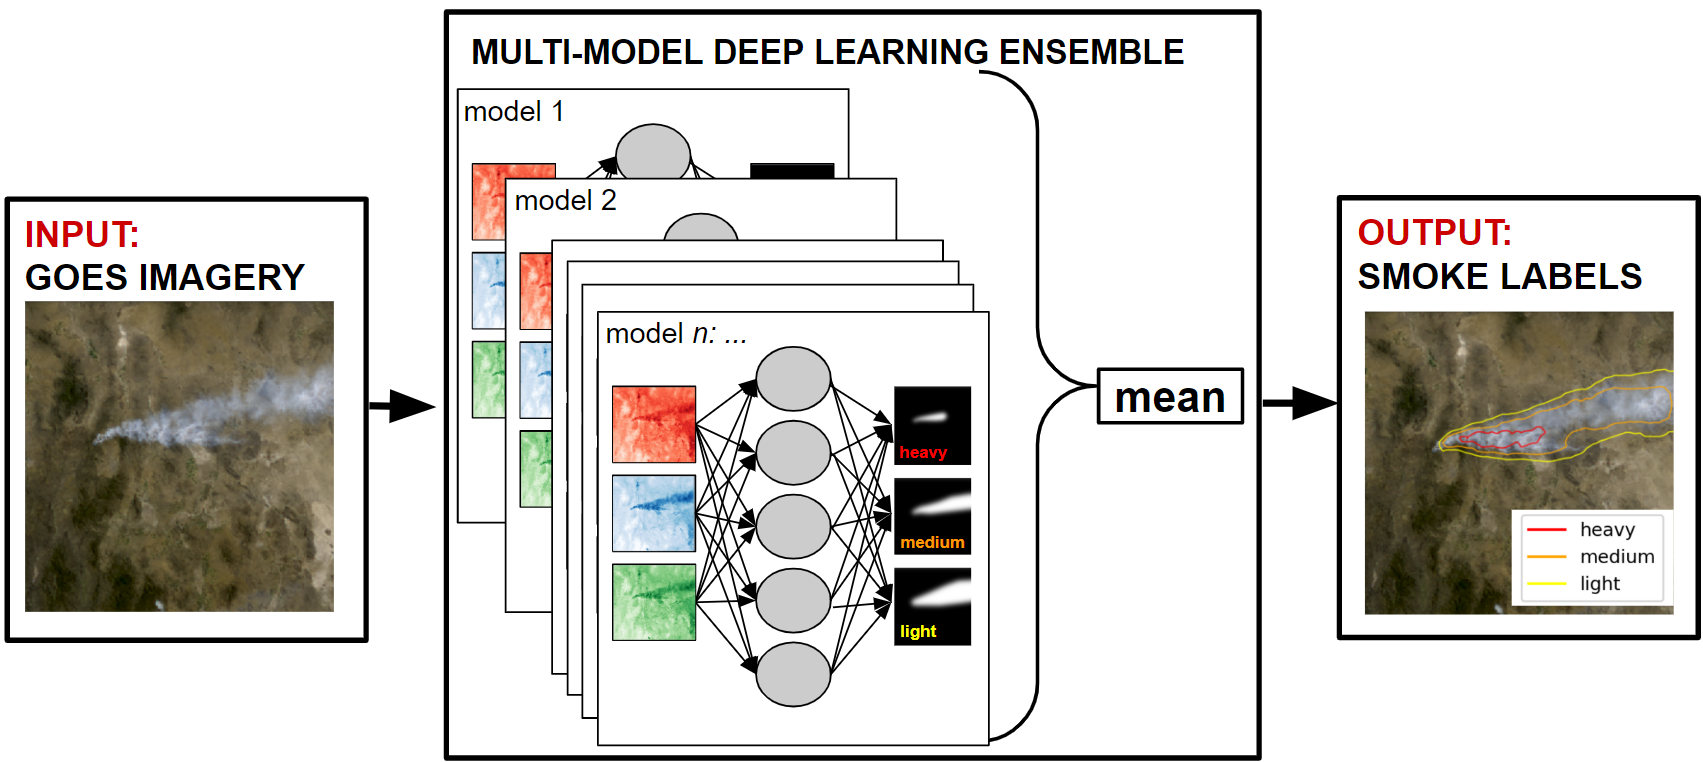
\includegraphics[width=0.75\textwidth]{ensemble_framework.png}
    \caption{Multi-Model Ensemble Framework.}
    \label{fig:ensemble_framework}
\end{figure}
\section{Results}
We measure model performance in terms of Intersection over Union (IoU) score (Equation \ref{overall_iou}) which quantifies the alignment between the model prediction ($ y^*_{i} $) and the ground truth ($y_{i}$). Table \ref{tab:results} shows the IoU scores for individual models and ensembles. The ensemble of 8 models with different architectures outperforms the individual models, with an improvement in the IoU score for all densities of smoke and over all densities. The ensemble of 8 models with different initial weights also outperforms the individual models, with a similar improvement in the IoU score. Figure \ref{fig:ensemble_size_plot} shows the IoU performance over all smoke densities as a function of ensemble size for the two ensemble schemes. The ensemble of 8 models with different initial weights improves with more models in the ensemble. This improvement is likely due to the different initializations allowing the models to search different parts of the parameter space and find different minima of the loss. The ensemble of 8 models with different architectures improves with more models in the ensemble up to 8 models, but then plateaus in performance. This plateau in performance could be due to the additional architectures not being as well suited for the task, or the models not having enough diversity in their errors to improve ensemble performance.

Figure \ref{fig:ensemble_panel} shows an example of smoke plume detection from the testing dataset. The ensemble predictions show smoother boundaries, making the prediction more comparable to the human-drawn polygon annotations.
\begin{equation} \label{overall_iou}
    \text{IoU}_{\text{overall}} = {\sum\limits_{i=\text{light}}^{\text{heavy}}|y_{i}\cap y^*_{i}|} \div {\sum\limits_{i=\text{light}}^{\text{heavy}}|y_{i}|\cup|y^*_{i}|}
\end{equation}
% \begin{equation} \label{overall_iou}
%     \text{IoU}_{\text{overall}} = \frac{\sum\limits_{i=\text{light}}^{\text{heavy}}|y_{i}\cap y^*_{i}|}{\sum\limits_{i=\text{light}}^{\text{heavy}}|y_{i}|\cup|y^*_{i}|}
% \end{equation}
\begin{table}[h]
    \centering
    \begin{tabular}{llrrr>{\bfseries}r}
        \hline
            &   Heavy &   Medium &   Light &   Overall \\
        \hline
         Single Model: DLV3P &   0.347 &     0.441 &  0.666 &      0.599  \\
         Single Model: PAN &  0.349 &     0.478 &  0.664 &      0.604 \\
        %  \rowcolor{gray!20}
         Architecture Ensemble (N=8) &   0.400 &     0.507 &  0.692 &      0.635 \\
        %  Architecture Ensemble (N=12) &  0.400 &     0.504 &  0.686 &      0.630 \\
         Random Initial Weights Ensemble (N=8) &  0.409 &     0.512 &  0.684 &      0.631 \\
        %  Random Initial Weights Ensemble (N=12) &   0.409 &     0.515 &  0.690 &      0.635 \\
         \hline
    \end{tabular}
    \caption{IoU results across three classes of smoke (light, medium, heavy) and over all densities. Presented for different individual models of different architectures (\citep{dlv3p}; \citep{PAN}), along with the archiecture-based ensemble and random initial weights ensemble performance, where N denotes the number of models in the ensemble.}
    \label{tab:results}
    \end{table}
\begin{figure}[h]
    \centering
    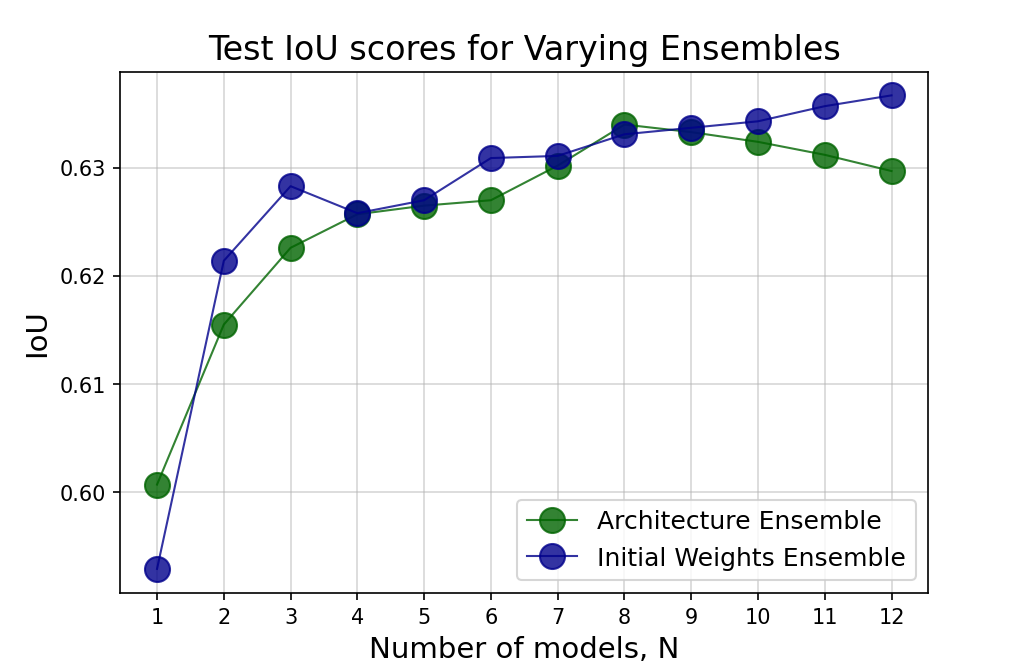
\includegraphics[width=0.75\textwidth]{ensemble_size_plot.png}
    \caption{Ensemble IoU Performance over all smoke densities as a function of ensemble size. Presented for two different schemes of ensemble design: random initial weights (blue) and architecure-based (red).}
    \label{fig:ensemble_size_plot}
\end{figure}
\begin{figure}[h]
    \centering
    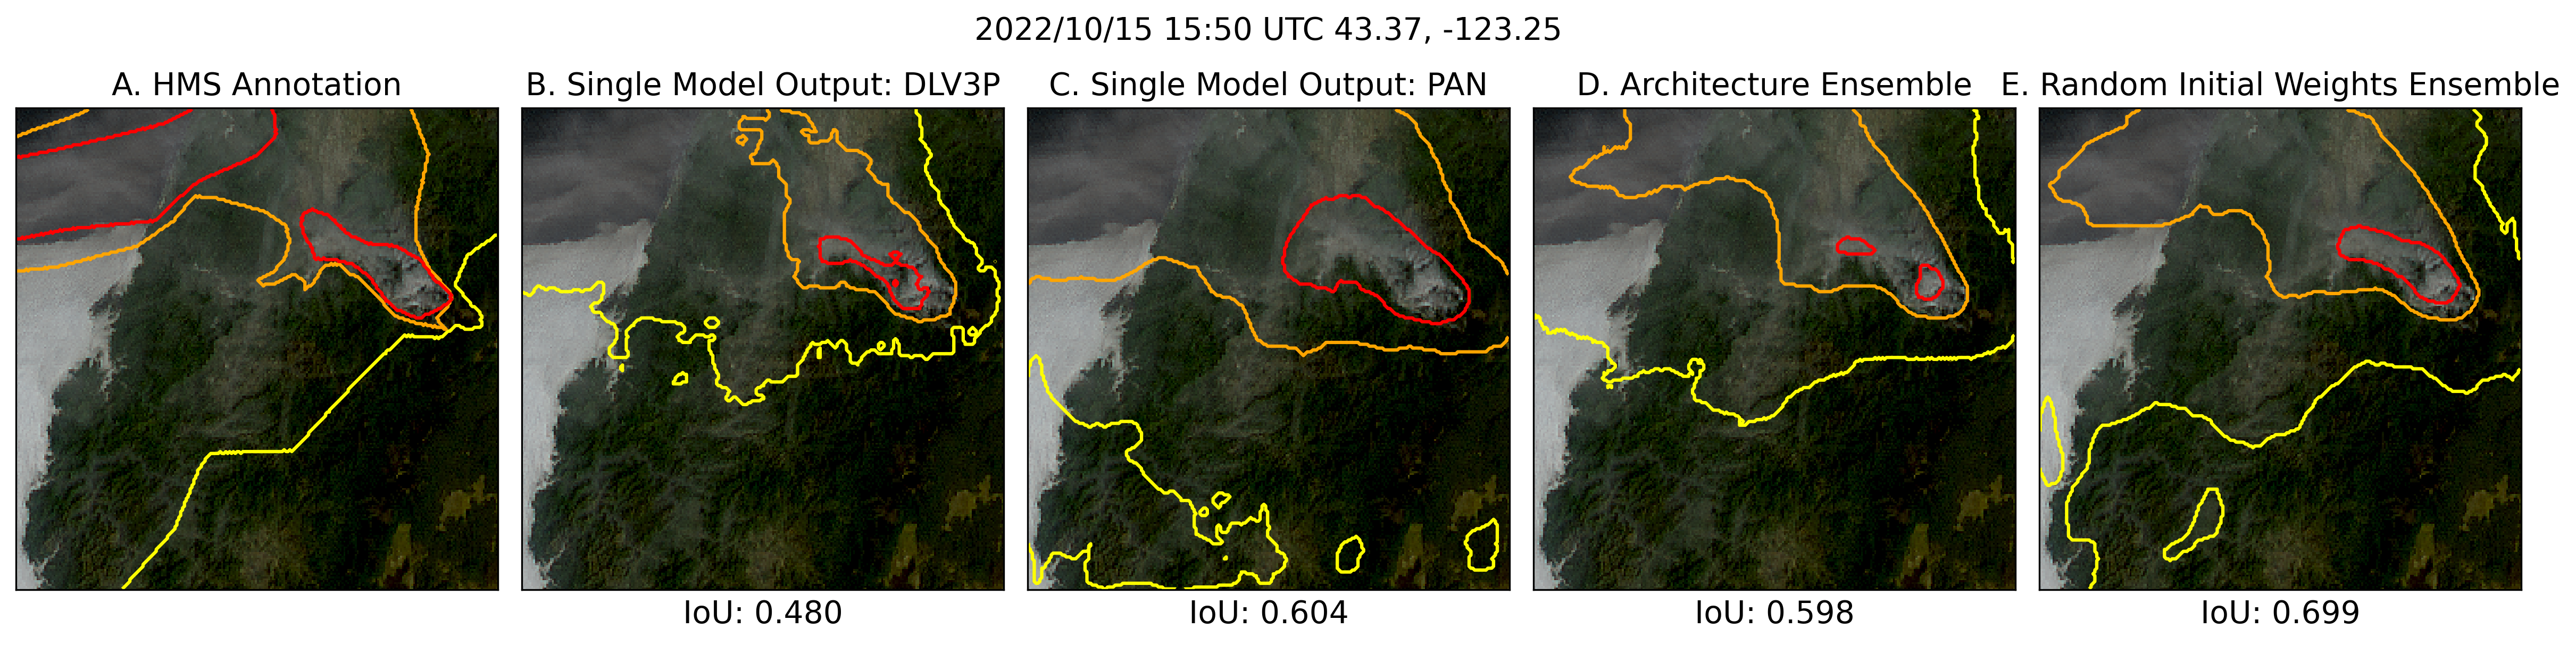
\includegraphics[width=\textwidth]{ensemble_panel_tinypaper.png}
    \caption{Example of smoke plume detection from GOES imagery with two individual models and two ensembles. Panel A displays the ground truth HMS annotation; Panels B-C show the predictions of two individual models; Panel D shows the prediction of an architecture-based ensemble of 8 models; Panel E shows the prediction of an ensemble made with 8 models with different random initial weights.}
    \label{fig:ensemble_panel}
\end{figure}
\section{Conclusions and Future Work}
We explored two schemes for making ensembles of deep learning models that both improve on testing set IoU and make the predictions more realistic. There is more to be investigates, such as why the architecture-based ensemble plateaus in performance after 8 models, and how a combination of the two ensemble schemes will perform. We are also experimenting with other ensemble techniques, such as regionally-trained models, to improve detection of smoke. The ensemble of deep learning models is expected to support fire and hazard management by automating the monitoring of smoke in real-time from satellite imagery. This tool can be used to provide more frequent and consistent detection of smoke plumes, ultimately supporting climate resilience and adaptation strategies.
\bibliographystyle{plainnat}
\bibliography{references}

% Tips for Submissions (from CCAI site):
% For examples of typical formatting and content, see submissions from our previous workshops.
% Be explicit: Describe how your proposed approach addresses climate change, demonstrating an understanding of the application area.
% Frame your work: The specific problem and/or data proposed should be contextualized in terms of prior work.
% Address the impact: Describe the practical implications of your method in addressing the problem you identify, as well as any relevant societal impacts or potential side-effects. We recommend reading our further guidelines on this aspect here.
% Explain the ML: Readers may not be familiar with the exact techniques you are using or may desire further detail.
% Justify the ML: Describe why the ML method involved is needed, and why it is a good match for the problem.
% Avoid jargon: Jargon is sometimes unavoidable but should be minimized. Ideal submissions will be accessible both to an ML audience and to experts in other relevant fields, without the need for field-specific knowledge. Feel free to direct readers to accessible overviews or review articles for background, where it is impossible to include context directly.
% Addressing Impact
% Tackling climate change requires translating ideas into action. The guidelines below will help you clearly present the importance of your work to a broad audience, hopefully including relevant decision-makers in industry, government, nonprofits, and other areas.

% Illustrate the link: Many types of work, from highly theoretical to deeply applied, can have clear pathways to climate impact. Some links may be direct, such as improving solar forecasting to increase utilization within existing electric grids. Others may take several steps to explain, such as improving computer vision techniques for classifying clouds, which could help climate scientists seeking to understand fundamental climate dynamics.
% Consider your target audience: Try to convey with relative specificity why and to whom solving the problem at hand will be useful. If studying extreme weather prediction, consider how you would communicate your key findings to a government disaster response agency. If analyzing a supply chain optimization pilot program, what are the main takeaways for industries who might adopt this technology? To ensure your work will be impactful, where possible we recommend co-developing projects with relevant stakeholders or reaching out to them early in the process for feedback. We encourage you to use this opportunity to do so!
% Outline key metrics: Quantitative or qualitative assessments of how well your results (or for proposals, anticipated results) compare to existing methods are encouraged. Try to give a sense of the importance of your problem and your findings. We encourage you to convey why the particular metrics you choose are relevant from a climate change perspective. For instance, if you are evaluating your machine learning model on the basis of accuracy, how does improved accuracy on a machine learning model translate to climate impact, and why is accuracy the best metric to use in this context?
% Be clear and concise: The discussion of impact does not need to be lengthy, just clear.
% Convey the big picture: Ultimately, the goal of Climate Change AI is to “empower work that meaningfully addresses the climate crisis.” Try to make sure that from the beginning, you contextualize your method and its impacts in terms of this objective
% In this case, IoU is the best metric because it directly reflects the model's ability to correctly identify smoke plumes, which is essential for making informed decisions in real-time scenarios.
% would omit iou but want to address the following: also dont want to throw numbers at people with no explanation, but am short on space. should i add the equation??? ***
% workshop site: Outline key metrics: Quantitative or qualitative assessments of how well your results (or for proposals, anticipated results) compare to existing methods are encouraged. Try to give a sense of the importance of your problem and your findings. We encourage you to convey why the particular metrics you choose are relevant from a climate change perspective. For instance, if you are evaluating your machine learning model on the basis of accuracy, how does improved accuracy on a machine learning model translate to climate impact, and why is accuracy the best metric to use in this context?
\end{document}